\documentclass[a4paper]{article}\usepackage[]{graphicx}\usepackage[]{color}
%% maxwidth is the original width if it is less than linewidth
%% otherwise use linewidth (to make sure the graphics do not exceed the margin)
\makeatletter
\def\maxwidth{ %
  \ifdim\Gin@nat@width>\linewidth
    \linewidth
  \else
    \Gin@nat@width
  \fi
}
\makeatother

\definecolor{fgcolor}{rgb}{0.345, 0.345, 0.345}
\newcommand{\hlnum}[1]{\textcolor[rgb]{0.686,0.059,0.569}{#1}}%
\newcommand{\hlstr}[1]{\textcolor[rgb]{0.192,0.494,0.8}{#1}}%
\newcommand{\hlcom}[1]{\textcolor[rgb]{0.678,0.584,0.686}{\textit{#1}}}%
\newcommand{\hlopt}[1]{\textcolor[rgb]{0,0,0}{#1}}%
\newcommand{\hlstd}[1]{\textcolor[rgb]{0.345,0.345,0.345}{#1}}%
\newcommand{\hlkwa}[1]{\textcolor[rgb]{0.161,0.373,0.58}{\textbf{#1}}}%
\newcommand{\hlkwb}[1]{\textcolor[rgb]{0.69,0.353,0.396}{#1}}%
\newcommand{\hlkwc}[1]{\textcolor[rgb]{0.333,0.667,0.333}{#1}}%
\newcommand{\hlkwd}[1]{\textcolor[rgb]{0.737,0.353,0.396}{\textbf{#1}}}%

\usepackage{framed}
\makeatletter
\newenvironment{kframe}{%
 \def\at@end@of@kframe{}%
 \ifinner\ifhmode%
  \def\at@end@of@kframe{\end{minipage}}%
  \begin{minipage}{\columnwidth}%
 \fi\fi%
 \def\FrameCommand##1{\hskip\@totalleftmargin \hskip-\fboxsep
 \colorbox{shadecolor}{##1}\hskip-\fboxsep
     % There is no \\@totalrightmargin, so:
     \hskip-\linewidth \hskip-\@totalleftmargin \hskip\columnwidth}%
 \MakeFramed {\advance\hsize-\width
   \@totalleftmargin\z@ \linewidth\hsize
   \@setminipage}}%
 {\par\unskip\endMakeFramed%
 \at@end@of@kframe}
\makeatother

\definecolor{shadecolor}{rgb}{.97, .97, .97}
\definecolor{messagecolor}{rgb}{0, 0, 0}
\definecolor{warningcolor}{rgb}{1, 0, 1}
\definecolor{errorcolor}{rgb}{1, 0, 0}
\newenvironment{knitrout}{}{} % an empty environment to be redefined in TeX

\usepackage{alltt}

\usepackage[english]{babel}
\usepackage[utf8]{inputenc}
\usepackage{amsmath}
\usepackage{amsfonts}
\usepackage{graphicx}
%\usepackage{fullpage}
%\usepackage{parskip}
\usepackage[round]{natbib}

% The line below tells R to use knitr on this.
%\VignetteEngine{knitr::knitr}

\newcommand{\boldbeta}{\boldsymbol{\beta}}
\newcommand{\Be}{\text{Bernoulli}}

\title{Bayesian Logistic Regression with Polya-Gamma latent variables}

\author{Kaspar Märtens \and Sherman Ip}
\IfFileExists{upquote.sty}{\usepackage{upquote}}{}
\begin{document}
\maketitle

\begin{abstract}
Your abstract.
\end{abstract}

\section{Introduction}

Motivation for Bayesian approach etc

\section{Data augmentation scheme}

In \cite{polson2013bayesian}, the Polya-Gamma family of distributions is carefully constructed so that introducing latent variables from this family yields a simple Gibbs sampler for the Bayesian logistic regression model.

Let
\[
y_i \sim \Be\left( \frac{1}{1 + \exp(-x_i^T \boldbeta)} \right)
\]
for data points $i=1, ..., N$, with $x_i$ the vector of covariates, and $\boldbeta$ the parameter vector with a prior distribution $\boldbeta \sim N(b, B)$. Sampling from the posterior distribution of $\boldbeta$ can be achieved by introducing the auxiliary random variables $\omega_i, i=1, ..., N$, and iterating the following two-step Gibbs sampling scheme:

\begin{enumerate}
\item $(\omega_i | \boldbeta) \sim PG(1, x_i^T \boldbeta)$
\item $(\boldbeta | y, \omega) \sim N(m_\omega, V_\omega)$
\end{enumerate}

where the first conditional distribution is a Polya-Gamma $PG(1, z)$ with some real number $z$, and the second one is a multivariate normal with the mean and covariance specified in \cite{polson2013bayesian}.
Note that there is a latent variable $\omega_i$ for each data point, i.e. the first step needs to be repeated $N$ times, whereas the parameters $\beta$ are sampled jointly.

One way for constructing a random variable $X$ from a Polya-Gamma distribution $PG(1, z)$ with $z \in \mathbb{R}$ is according to the definition, i.e.
\[
X \gets \sum_{k=1}^\infty \frac{g_k}{(k-0.5)^2 + \frac{z^2}{4 \pi^2}}
\]
where $g_k \sim \Gamma(1, 1)$ are i.i.d. random variables. The definition contains an infinite sum and it is not clear how its truncation to a finite number of terms will affect the results.

Instead, an accept-reject sampling procedure is proposed to sample from $PG(1,z)$.

\section{Implementation}

\subsection{Gibbs sampling}

\subsection{Sampling from the Polya-Gamma distribution}

\begin{figure}
\centering
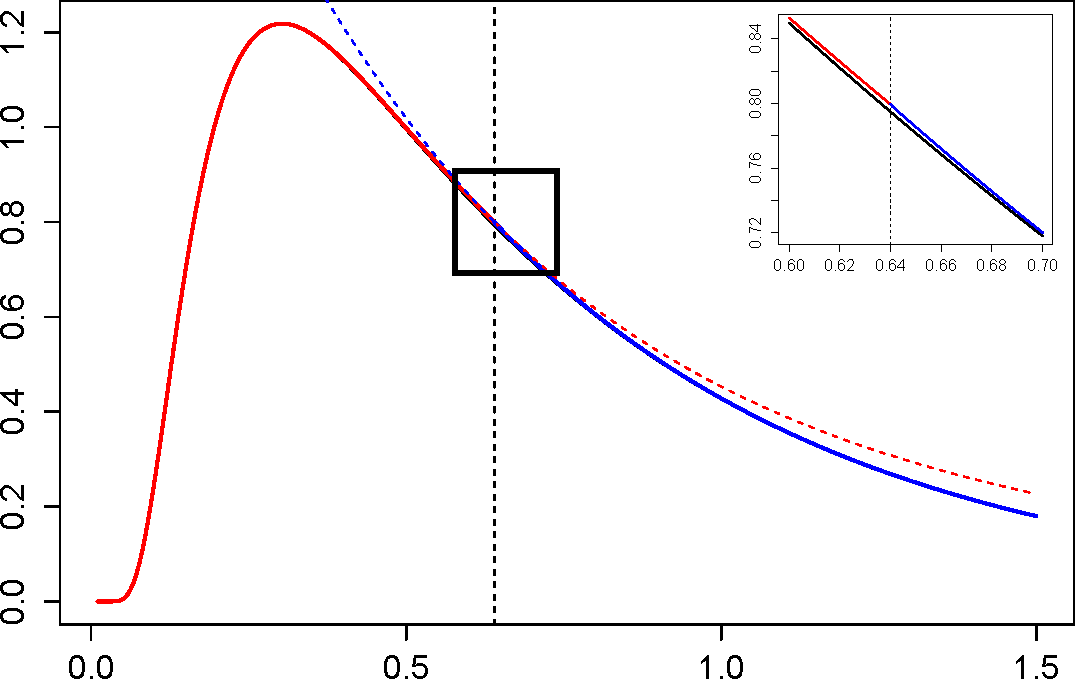
\includegraphics[width=0.6\textwidth]{fig/fig_accept_reject_final}
\caption{Visualisation of the accept-reject algorithm for the target PG(1, 1) distribution (density in black). The proposal distribution is defined in two pieces: for $x \in (0, 0.64]$ (density in red) and $x \in (0.64, \infty)$ (blue). The middle portion of the figure has been zoomed in (top right corner). The dashed lines (red and blue) extend the densities of proposal distributions outside their defined range.}
\end{figure}

%\subsubsection{Naive approach}
%\subsubsection{Accept-reject algorithm}

\section{Experiments and results}

\subsection{Tests on simulated data}

\subsubsection{???}

\begin{figure}[ht]
\centering
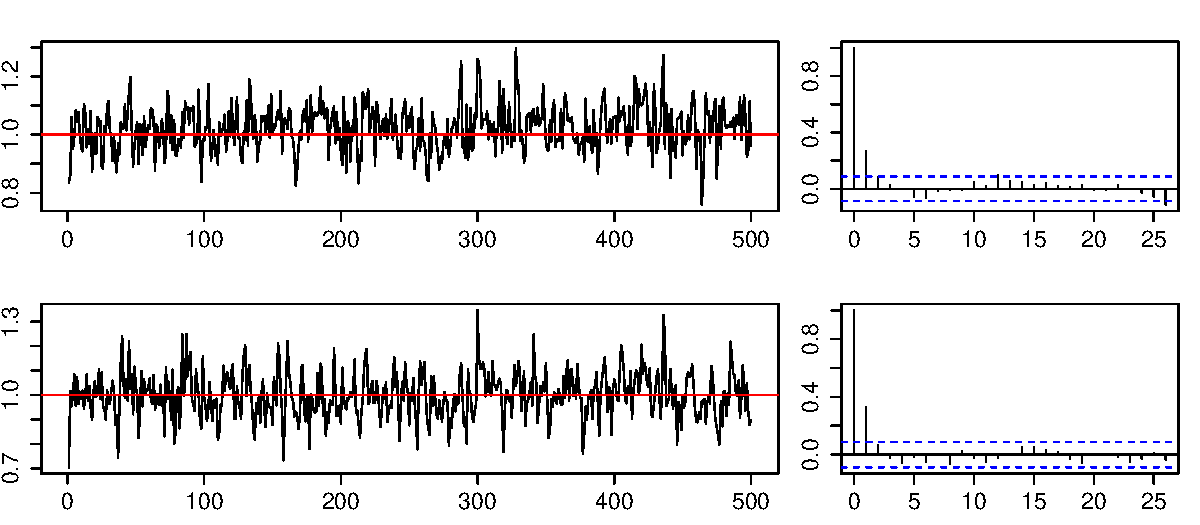
\includegraphics[width=0.8\textwidth]{fig/fig_traceplot_beta}
\caption{Traceplot of $\beta_1$ on simulated data }
\end{figure}



\begin{knitrout}
\definecolor{shadecolor}{rgb}{0.969, 0.969, 0.969}\color{fgcolor}\begin{kframe}
\begin{alltt}
\hlstd{devtools}\hlopt{::}\hlkwd{load_all}\hlstd{()}
\end{alltt}


{\ttfamily\noindent\itshape\color{messagecolor}{\#\# Loading PolyaGamma}}\begin{alltt}
\hlstd{data} \hlkwb{=} \hlkwd{generate_from_simple_logistic_model}\hlstd{(}\hlnum{1000}\hlstd{)}
\hlstd{obj} \hlkwb{=} \hlkwd{gibbs_sampler}\hlstd{(data}\hlopt{$}\hlstd{y, data}\hlopt{$}\hlstd{X,} \hlkwc{lambda} \hlstd{=} \hlnum{0.01}\hlstd{,} \hlkwc{n_iter} \hlstd{=} \hlnum{100}\hlstd{)}
\hlkwd{plot}\hlstd{(obj)}
\end{alltt}
\end{kframe}
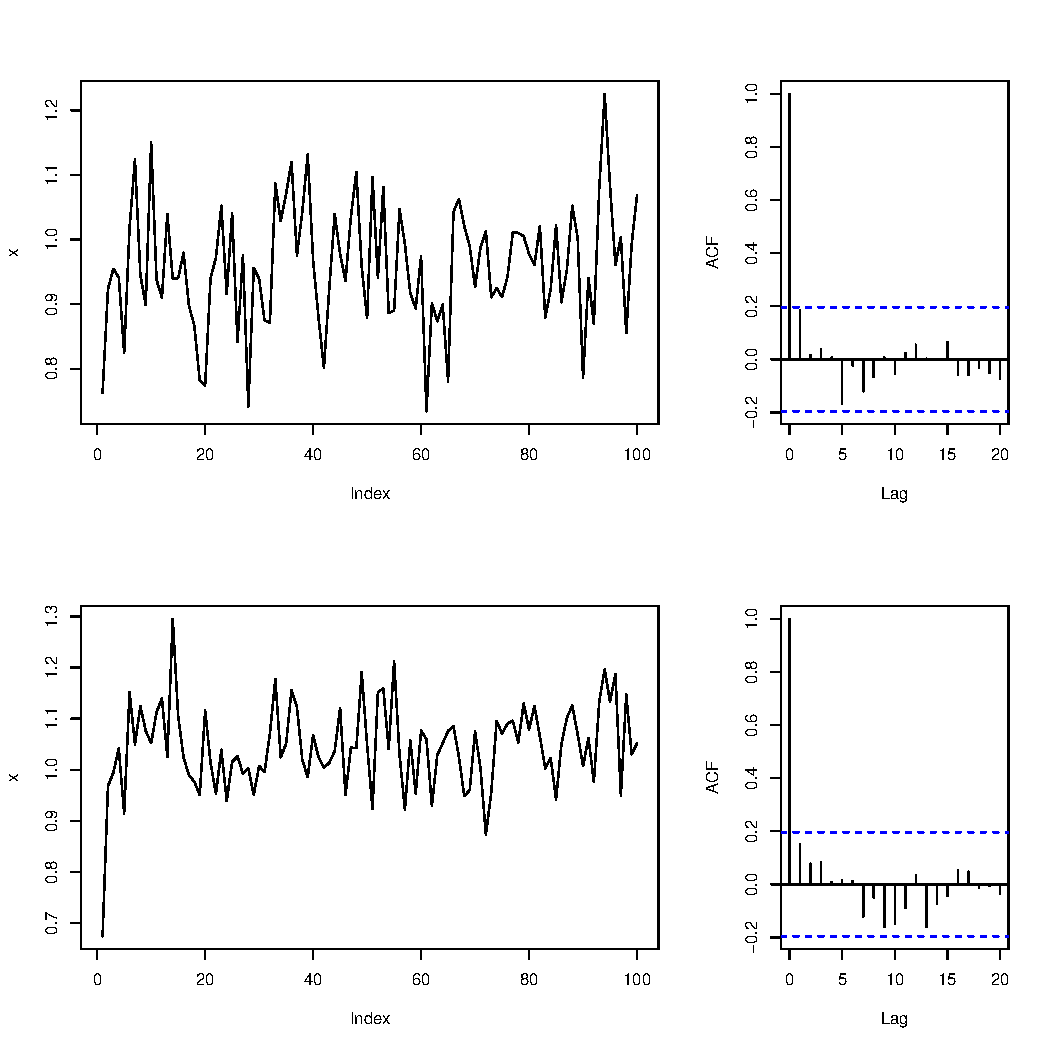
\includegraphics[width=\maxwidth]{figure/unnamed-chunk-1-1} 

\end{knitrout}

say something about the posterior distribution of beta

effective sample size??

\begin{figure}[ht]
\centering
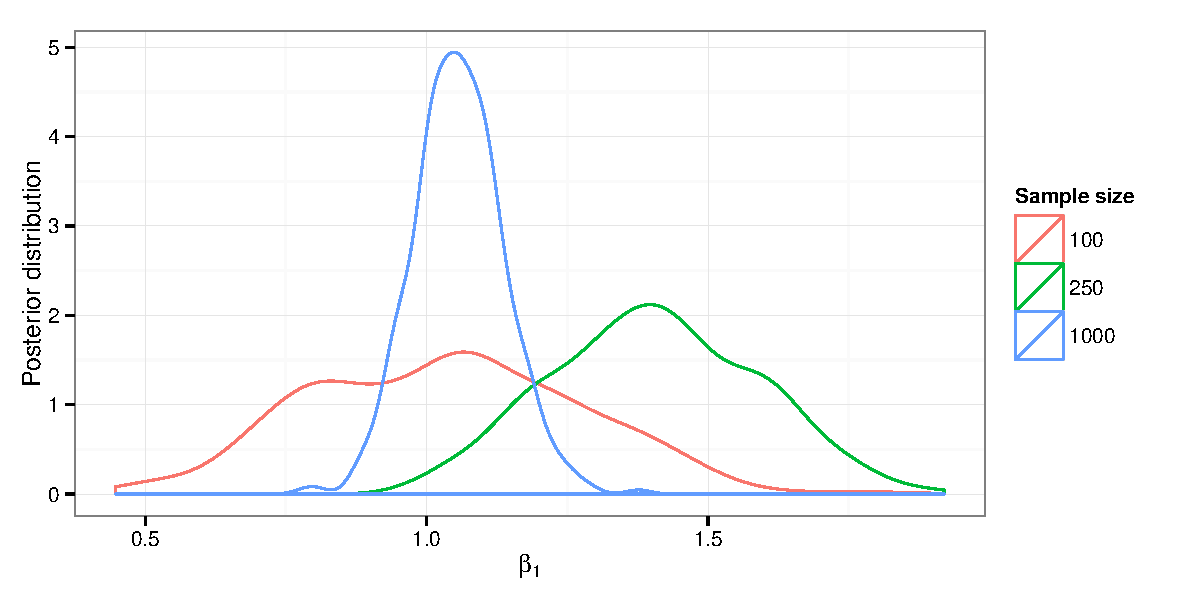
\includegraphics[width=0.7\textwidth]{fig/posterior_with_different_n}
\caption{Posterior distribution (smoothed histograms) of $\beta_1$ for different sample sizes.}
\end{figure}

\subsubsection{Efficient sampling from Polya-Gamma distribution}

Compare the naive approach versus accept-reject algorithm (autocorrelations, computation time)

\subsubsection{Comparison with BayesLogit package}

check that the results are the same, compare computation time

\subsection{Tests on real data}

\section{Future work?}


\bibliographystyle{plainnat}
\bibliography{mybib}

\end{document}
